\documentclass[12pt]{article}
\usepackage[utf8]{inputenc}
\usepackage[legalpaper, margin=0.5in]{geometry}
\usepackage{listings}
\usepackage{xcolor}
\usepackage{graphicx}
\usepackage{amsmath}

\setlength{\parindent}{0em}
\setlength{\parskip}{1em}

%New colors defined below
\definecolor{codegreen}{rgb}{0,0.6,0}
\definecolor{codegray}{rgb}{0.5,0.5,0.5}
\definecolor{codepurple}{rgb}{0.58,0,0.82}
\definecolor{backcolour}{rgb}{0.95,0.95,0.95}

%Code listing style named "mystyle"
\lstdefinestyle{mystyle}{
  backgroundcolor=\color{backcolour},   commentstyle=\color{codegreen},
  keywordstyle=\color{magenta},
  numberstyle=\tiny\color{codegray},
  stringstyle=\color{codepurple},
  basicstyle=\ttfamily\normalsize,
  breakatwhitespace=false,         
  breaklines=true,                 
  captionpos=b,                    
  keepspaces=true,                 
  numbersep=5pt,                  
  showspaces=false,                
  showstringspaces=false,
  showtabs=false,                  
  tabsize=2
}

%"mystyle" code listing set
\lstset{style=mystyle}

\graphicspath{{resources/}}

\title{Lesson 8: Gradients and Color Spaces}
\author{Jinil Jang }
\date{October 2019}

\begin{document}

\maketitle

\section{Sobel Operator}

The Sobel operator is at the heart of the Canny edge detection algorithm. Applying the Sobel operator to an image is a way of taking the derivative of the image in the $x$ and $y$ direction. This is example of Sobel operators with a kernel size of 3. The kernel size can be any odd number.

$$S_x = 
\begin{vmatrix}
-1&0&1\\
-2&0&2\\
-1&0&1\\
\end{vmatrix}
$$

$$S_y = 
\begin{vmatrix}
-1&-2&-1\\
0&0&0\\
1&2&1\\
\end{vmatrix}
$$

If the image is flat across the region (i.e., there is little change in values across the given region), then the result(summing the element-wise product of the operator and corresponding image pixels) will be zero.

$$gradient = \sum (region * S_x)$$

To use the \textbf{cv2.Sobel()}, a single color channel should be passed.

\begin{lstlisting}[language=Python]
gray = cv2.cvtColor(im, cv2.COLOR_RGB2GRAY)
\end{lstlisting}

\textbf{Note: } \\
Use \textbf{cv2.COLOR\_RGB2GRAY} if you've read in an image using \textbf{mpimg.imread()}. \\
Use \textbf{cv2.COLOR\_BGR2GRAY} if you've read in an image using \textbf{cv2.imread()}.

Calculate the derivative in the x direction (the 1, 0 at the end denotes $x$ direction)

\begin{lstlisting}[language=Python]
sobelx = cv2.Sobel(gray, cv2.CV_64F, 1, 0)
\end{lstlisting}

Calculate the derivative in the y direction (the 0, 1 at the end denotes $y$ direction)

\begin{lstlisting}[language=Python]
sobely = cv2.Sobel(gray, cv2.CV_64F, 0, 1)
\end{lstlisting}

Calculate the absolute value of the $x$ derivative

\begin{lstlisting}[language=Python]
abs_sobelx = np.absolute(sobelx)
\end{lstlisting}

Convert the absolute value image to 8-bit

\begin{lstlisting}[language=Python]
scaled_sobel = np.uint8(255 * abs_sobelx / np.max(abs_sobelx))
\end{lstlisting}

Create a binary threshold to select pixels based on gradient strength

\begin{lstlisting}[language=Python]
thresh_min = 20
thresh_max = 100
sxbinary = np.zeros_like(scaled_sobel)
sxbinary[(scaled_sobel >= thresh_min) & (scaled_sobel <= thresh_max)] = 1
plt.imshow(sxbinary, cmap='gray')
\end{lstlisting}

\begin{figure}[htp]
    \centering
    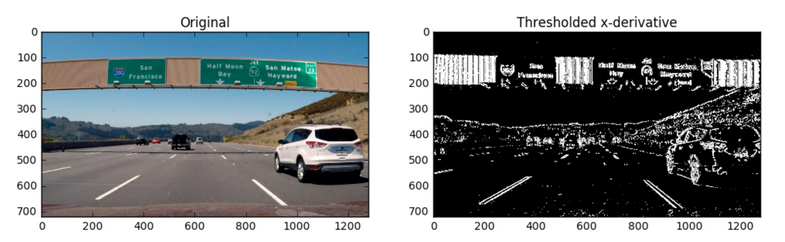
\includegraphics[width=15cm]{sobel_x.png}
    \label{fig:sobel_x}
\end{figure}

\begin{figure}[htp]
    \centering
    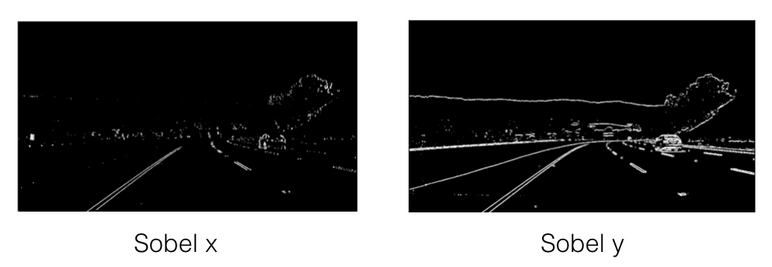
\includegraphics[width=15cm]{sobel_x_y.png}
    \label{fig:sobel_x_y}
\end{figure}

\section{Magnitude of the Gradient}

$$abs\_sobelx = \sqrt{(sobel_x)^2}$$
$$abs\_sobely = \sqrt{(sobel_y)^2}$$
$$abs\_sobelxy = \sqrt{(sobel_x)^2 + (sobel_y)^2}$$

\begin{lstlisting}[language=Python]
import numpy as np
import cv2
import matplotlib.pyplot as plt
import matplotlib.image as mpimg
import pickle

# Read in an image
image = mpimg.imread('signs_vehicles_xygrad.png')

# Define a function that applies Sobel x and y, 
# then computes the magnitude of the gradient
# and applies a threshold
def mag_thresh(img, sobel_kernel=3, mag_thresh=(0, 255)):
    
    # Apply the following steps to img
    # 1) Convert to grayscale
    gray = cv2.cvtColor(img, cv2.COLOR_RGB2GRAY)
    
    # 2) Take the gradient in x and y separately
    sobelx = cv2.Sobel(gray, cv2.CV_64F, 1, 0, ksize=sobel_kernel)
    sobely = cv2.Sobel(gray, cv2.CV_64F, 0, 1, ksize=sobel_kernel)
    
    # 3) Calculate the magnitude 
    abs_sobelxy = np.sqrt(sobelx**2 + sobely**2)
    
    # 4) Scale to 8-bit (0 - 255) and convert to type = np.uint8
    scaled_sobel = np.uint8(255 * abs_sobelxy / np.max(abs_sobelxy))
    
    # 5) Create a binary mask where mag thresholds are met
    binary_output = np.zeros_like(scaled_sobel)
    binary_output[(scaled_sobel >= mag_thresh[0]) & (scaled_sobel <= mag_thresh[1])] = 1
    
    # 6) Return this mask as your binary_output image
    return binary_output
    
# Run the function
mag_binary = mag_thresh(image, sobel_kernel=3, mag_thresh=(30, 100))
# Plot the result
f, (ax1, ax2) = plt.subplots(1, 2, figsize=(24, 9))
f.tight_layout()
ax1.imshow(image)
ax1.set_title('Original Image', fontsize=50)
ax2.imshow(mag_binary, cmap='gray')
ax2.set_title('Thresholded Magnitude', fontsize=50)
plt.subplots_adjust(left=0., right=1, top=0.9, bottom=0.)
\end{lstlisting}

\begin{figure}[htp]
    \centering
    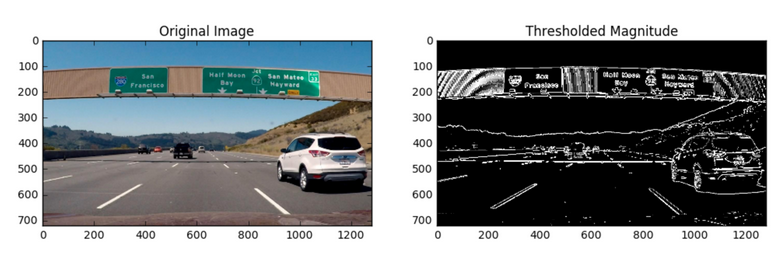
\includegraphics[width=15cm]{magnitute_gradient.png}
    \label{fig:magnitute_gradient}
\end{figure}

\section{Direction of the Gradient}

Direction of the gradient is the inverse tangent (arctangent) of the $y$ gradient divided by the $x$ gradient

$$arctan(sobel_y/sobel_x)$$

\begin{lstlisting}[language=Python]
# Define a function that applies Sobel x and y, 
# then computes the direction of the gradient
# and applies a threshold.
def dir_threshold(img, sobel_kernel=3, thresh=(0, np.pi/2)):
    
    # Apply the following steps to img
    # 1) Convert to grayscale
    gray = cv2.cvtColor(img, cv2.COLOR_RGB2GRAY)
    
    # 2) Take the gradient in x and y separately
    sobelx = cv2.Sobel(gray, cv2.CV_64F, 1, 0, ksize=sobel_kernel)
    sobely = cv2.Sobel(gray, cv2.CV_64F, 0, 1, ksize=sobel_kernel)
    
    # 3) Take the absolute value of the x and y gradients
    abs_sobelx = np.absolute(sobelx)
    abs_sobely = np.absolute(sobely)
    
    # 4) Use np.arctan2(abs_sobely, abs_sobelx) to calculate the direction of the gradient 
    absgraddir = np.arctan2(abs_sobely, abs_sobelx)
    
    # 5) Create a binary mask where direction thresholds are met
    binary_output = np.zeros_like(absgraddir)
    binary_output[(absgraddir >= thresh[0]) & (absgraddir <= thresh[1])] = 1
    
    # 6) Return this mask as your binary_output image
    return binary_output
\end{lstlisting}

\begin{figure}[htp]
    \centering
    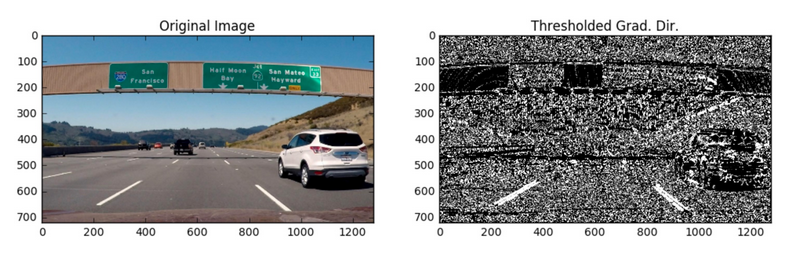
\includegraphics[width=15cm]{direction_of_gradient.png}
    \label{fig:direction_of_gradient}
\end{figure}

\section{Color Thresholding}

\subsection{HSV}

Hue, Saturation, and Value

\textbf{Hue}\\
The value that represents color independent of any change in brightness.
So if you imagine a basic red paint color, then add some white to it or some black to make that color lighter or darker -- the underlying color remains the same and the hue for all of these colors will be the same. 

\textbf{Saturation}\\
Measurement of colorfulness. So, as colors get lighter and closer to white, they have a lower saturation value, whereas colors that are the most intense, like a bright primary color (imagine a bright red, blue, or yellow), have a high saturation value.

\subsection{HLS}

Hue, Lightness, and Saturation

\textbf{Lightness} and \textbf{Value}\\
Measure the relative lightness or darkness of a color. For example, a dark red will have a similar hue but much lower value for lightness than a light red.

\begin{figure}[htp]
    \centering
    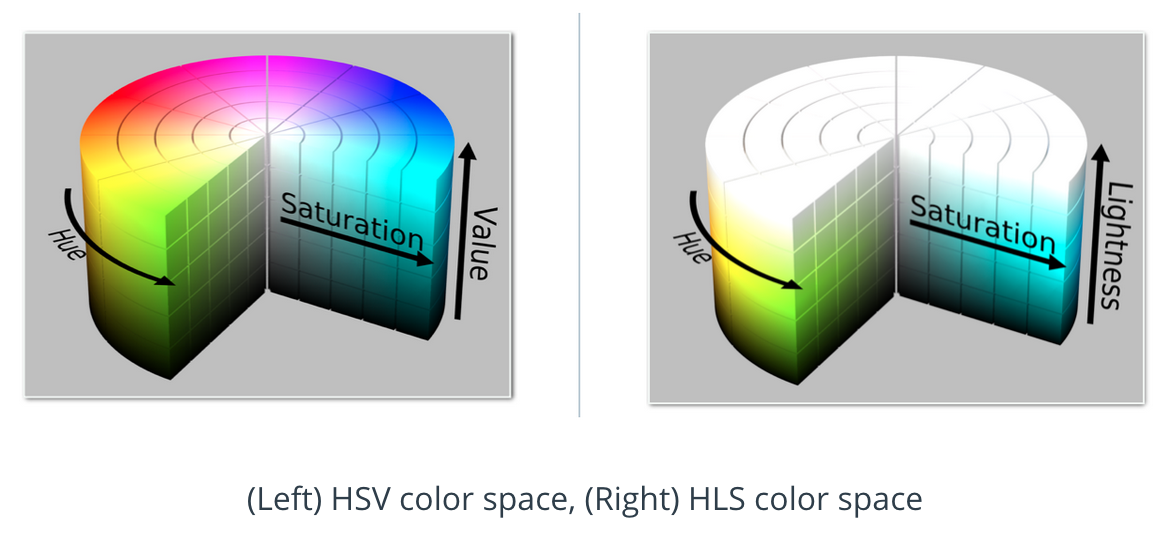
\includegraphics[width=10cm]{hsv_hls_color_space.png}
    \label{fig:hsv_hls_color_space}
\end{figure}

\section{Convert Color Space}

\textbf{OpenCV}

\begin{lstlisting}[language=Python]
hls = cv2.cvtColor(im, cv2.COLOR_RGB2HLS)
\end{lstlisting}

\textbf{Calculation}

$$V_{max} \leftarrow max(R, G, B)$$
$$V_{min} \leftarrow min(R, G, B)$$

\textbf{H} channel conversion equations

$$H \leftarrow \frac{30(G-B)}{V_{max}-V_{min}}, if V_{max} = R$$
$$H \leftarrow 60 + \frac{30(B-R)}{V_{max}-V_{min}}, if V_{max} = G$$
$$H \leftarrow 120 + \frac{30(R-G)}{V_{max}-V_{min}}, if V_{max} = B$$

\textbf{L} channel conversion equation

$$L \leftarrow \frac{V_{max} + V_{min}}{2}$$

\textbf{S} channel conversion equations

$$S \leftarrow \frac{V_{max} - V_{min}}{V_{max} + V_{min}}, if L < 0.5$$
$$S \leftarrow \frac{V_{max} - V_{min}}{2 - (V_{max} + V_{min})}, if L \geq 0.5$$

\section{HLS and Color Thresholds}

\begin{lstlisting}[language=Python]
hls = cv2.cvtColor(image, cv2.COLOR_RGB2HLS)
H = hls[:,:,0]
L = hls[:,:,1]
S = hls[:,:,2]

thresh = (90, 255)
binary = np.zeros_like(S)
binary[(S > thresh[0]) & (S <= thresh[1])] = 1
\end{lstlisting}

\section{Combine color and gradient}

\begin{lstlisting}[language=Python]
# Convert to HLS color space and separate the S channel
# Note: img is the undistorted image
hls = cv2.cvtColor(img, cv2.COLOR_RGB2HLS)
s_channel = hls[:,:,2]

# Grayscale image
# NOTE: we already saw that standard grayscaling lost color information for the lane lines
# Explore gradients in other colors spaces / color channels to see what might work better
gray = cv2.cvtColor(img, cv2.COLOR_RGB2GRAY)

# Sobel x
sobelx = cv2.Sobel(gray, cv2.CV_64F, 1, 0) # Take the derivative in x
abs_sobelx = np.absolute(sobelx) # Absolute x derivative to accentuate lines away from horizontal
scaled_sobel = np.uint8(255*abs_sobelx/np.max(abs_sobelx))

# Threshold x gradient
thresh_min = 20
thresh_max = 100
sxbinary = np.zeros_like(scaled_sobel)
sxbinary[(scaled_sobel >= thresh_min) & (scaled_sobel <= thresh_max)] = 1

# Threshold color channel
s_thresh_min = 170
s_thresh_max = 255
s_binary = np.zeros_like(s_channel)
s_binary[(s_channel >= s_thresh_min) & (s_channel <= s_thresh_max)] = 1

# Stack each channel to view their individual contributions in green and blue respectively
# This returns a stack of the two binary images, whose components you can see as different colors
color_binary = np.dstack(( np.zeros_like(sxbinary), sxbinary, s_binary)) * 255

# Combine the two binary thresholds
combined_binary = np.zeros_like(sxbinary)
combined_binary[(s_binary == 1) | (sxbinary == 1)] = 1
\end{lstlisting}

\begin{figure}[htp]
    \centering
    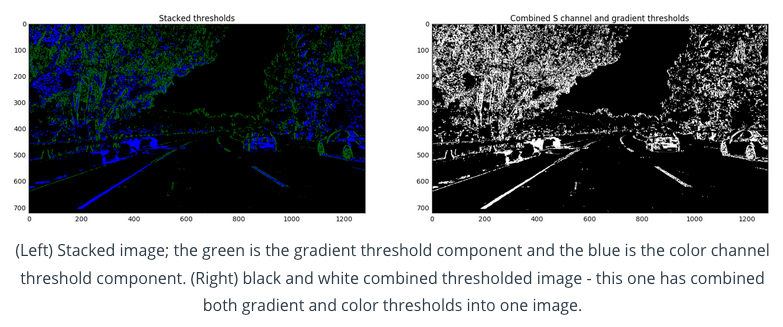
\includegraphics[width=15cm]{color_gradient.png}
    \label{fig:color_gradient}
\end{figure}

\end{document}